\chapter{Procedures for Aerodrome Control Service}

\section{Clearance}

An IFR clearance consists of:
\begin{itemize}
    \item aircraft identification,
    \item clearance limit (usually the destination aerodrome),
    \item designator of the assigned SID, if applicable,
    \item initial level, except when it is included in the SID description,
    \item squawk code,
    \item other necessary instructions or information not contained in the SID description.
\end{itemize}

Checking flight plan's correctness includes:
\begin{itemize}
    \item verifying the departure and arrival aerodromes have been filled correctly,
    \item checking if the cruising level filed is correct according to the semi-circular rule,
    \item checking the flight planned route up to the FIR boundary,
    \item analysis of the remarks.
\end{itemize}

\section{Start-up and pushback}

Start-up and pushback can be conducted, when:
\begin{itemize}
    \item crew reports ready for start-up/pushback,
    \item there is no traffic moving behind the aircraft,
    \item the clearance will not hinder the traffic flow.
\end{itemize}

Detailed local procedures regarding start-up and pushback are described in the appropriate sections.

\section{Taxi}

Taxi instructions shall be issued in such a way, that:
\begin{itemize}
    \item taxi routes of aircraft do not cross, unless proper conditional instructions have been issued,
    \item manouvering area occupancy has been reduced to minimum, i.e.\ the taxi route should be the shortest available,
    \item issued instructions do not violate or create a risk of unauthorized incursion onto an active runway, 
    \item maintain appropriate buffers around active runway holding points: used to occupy and vacate the runway so as not to block the movement of aircraft occupying or vacating the runway.
\end{itemize}

\section{Runway operations}
\subsubsection{Selecting runway in use}

Runway in use shall be selected using the following Runway Selection Preference System:
\begin{enumerate}
    \item Wind speed
    \begin{table}[htb]
        \centering
        %\rowcolors{2}{vpink}{white}
        \begin{tabular}{|M{2.5cm}|M{15cm}|}
            \rowcolor{vred}
            \color{white}\textbf Wind Speed & \color{white}\textbf Runway in use \\\hline
            0 --- 5 kts & Not dependent on wind direction\\\hline
            6 --- 15 kts & Closest ``into the wind'', unless other meteorological conditions determine otherwise\\\hline
            > 16 kts or gusts > 20 kts & ``Into the wind'', disregarding other meteorological conditions\\\hline
        \end{tabular}
        \caption{Runway Selection Preference System}
        \label{tbl:runwaySelect}
    \end{table}
    \item Available instrument procedures
    
    Better equipped runways should be selected first, in sequence:
    \begin{itemize}
        \item available LVP procedures (ILS CAT II/III, RNP AR APCH),
        \item available precision approach procedures (ILS, PAR),
        \item available non-precision approach procedures (VOR, TACAN, RNP, NDB),
        \item available visual aids (PAPI, runway lights, approach lights).
    \end{itemize}
    \item Runway conditions
    \item Safety considerations
\end{enumerate}

\subsubsection{Lining up and vacating runways}

Line up instruction may only be given if no clearance has been given to another aircraft to use the runway for take-off or landing. The exception is a conditional instruction, provided that the aircraft crew confirms that it can be carried out (e.g.\ reporting traffic in sight).
The runway may also be occupied when another aircraft is moving on it and is not performing the above-mentioned operations (e.g.\ taxiing, crossing the runway, finishing its landing roll, etc.).

Lining up and departing from a shortened take-off distance requires flight crew approval, unless local procedures say otherwise.

The runway is considered vacated when the aircraft has completely passed the stop bar/holding point.

\subsubsection{Operations from a runway other than runway in use}

Operations from a runway other than the runway in use require coordination with the controller responsible for providing approach control service for the aerodrome.

\section{Departure}

Clearance for take-off may only be issued when no other aircraft is in front of the taking-off aircraft on the runway.

Take-off clearance may be issued to an aircraft when there is reasonable assurance that the required separation  will exist when the aircraft commences take-off.

For departures that come under the responsibility of an approach/area controller after departure, take-off clearance can be issued only if the approach/area control unit authorizes the take-off (grants a \emph{``departure release''}), unless local procedures or coordination indicate otherwise.

Final positions that must be reached by arriving aircraft \emph{(A)} or departing aircraft \emph{(B or C)} before an arriving aircraft can be cleared to land of a runway in use or a departing aircraft can be cleared for take-off:

\begin{figure}[htbp]
    \centering
    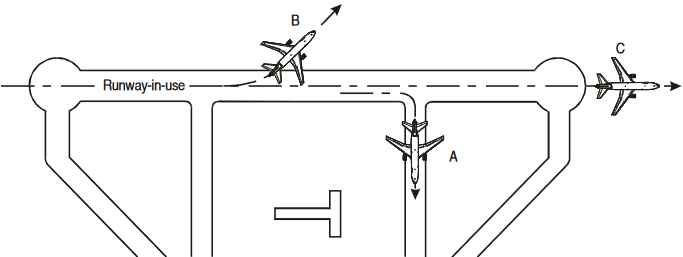
\includegraphics[width=0.8\textwidth]{4444/fig7-3.png}
    \caption{Separation between departing and arriving aircraft~\cite{4444}}
    \label{fig:separation_between_dep_and_arr}
\end{figure}

\clearpage
Separation of departing aircraft:
\begin{itemize}
    \item based on a surveillance system:
    \begin{itemize}
        \item 3~NM --- departures in different directions/different SIDs,
        \item 5~NM --- departures in the same direction/same SIDs,
        \item 5~NM --- departures in different directions/different SIDs, when the Preceding aircraft is 40~kts or more slower than the succeeding aircraft,
    \end{itemize}
    \item based on time:
    \begin{itemize}
        \item 5~minutes --- between departing aircraft on the same track, if the following aircraft will be crossing the level of the Preceding aircraft,
        \begin{figure}[htbp]
            \centering
            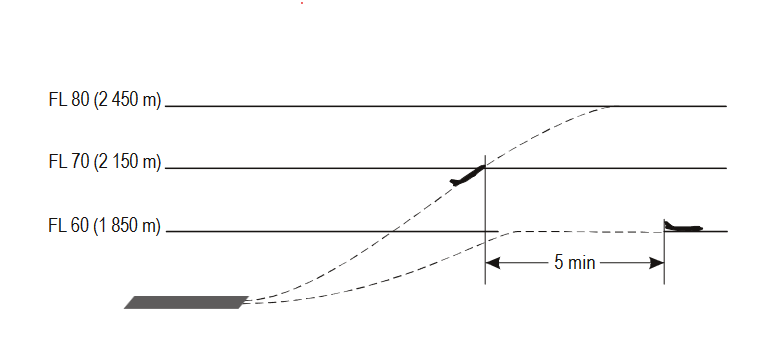
\includegraphics[width=0.5\textwidth]{4444/fig5-37.png}
            \caption{Five-minute separation of departing aircraft following the same track~\cite{4444}}
            \label{fig:5min_departures}
        \end{figure}
        \item 2~minutes --- between departing aircraft on the same track, when the Preceding aircraft is at least 40 kts faster,
        \begin{figure}[htbp]
            \centering
            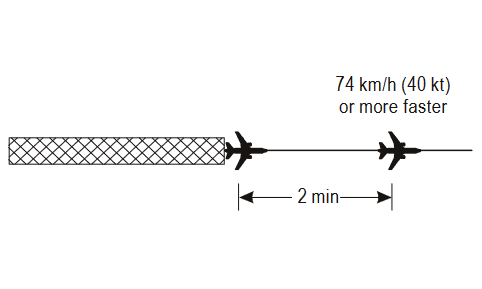
\includegraphics[width=0.5\textwidth]{4444/fig5-36.png}
            \caption{Two-minute separation between aircraft following same track~\cite{4444}}
            \label{fig:2min_departures}
        \end{figure}
        \item 1~minute --- between departing aircraft, when their departure tracks differ by no less than 45{\degree},
        \begin{figure}[htbp]
            \centering
            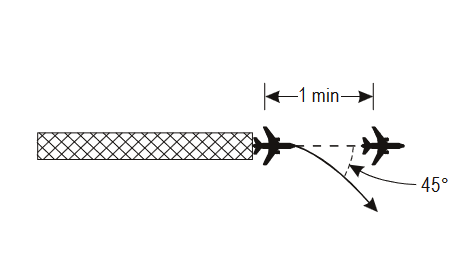
\includegraphics[width=0.5\textwidth]{4444/fig5-35.png}
            \caption{One-minute separation between departing aircraft following tracks diverging by at least 45\degree~\cite{4444}}
            \label{fig:1min_departures}
        \end{figure}
    \end{itemize}
    \item based on visual observation \emph{(VFR)}:
    \begin{itemize}
        \item aircraft has started a turn or passed departure end of the runway.
    \end{itemize}
\end{itemize}

Departures from intersecting runways are subject to common departure separations (requires usage of same separations as departures from the same runway).

\subsubsection{Wake turbulence separation --- departures}

In addition to standard established separations, an important factor is the consideration of wake turbulence of departing aircraft of different categories:

The same starting point of the take-off run:
\begin{table}[htbp]
    \centering
    \begin{tabular}{|M{3cm}|M{3cm}|M{3cm}|}
        \hline\rowcolor{vred}
        \color{white}\textbf{Preceding} & \color{white}\textbf{Succeeding} & \color{white}\textbf{Separation}\\\hline
        SUPER (J) & HEAVY (H) & 2 min\\\hline
        SUPER (J) & \multirow{2}{*}{MEDIUM (M)} & 3 min\\\cline{1-1}\cline{3-3}
        HEAVY (H) & & 2 min\\\hline
        SUPER (J) & \multirow{3}{*}{LIGHT (L)} & 3 min\\\cline{1-1}\cline{3-3}
        MEDIUM (M) & & \multirow{2}{*}{2 min}\\\cline{1-1}
        LIGHT & &\\\hline
    \end{tabular}
    \caption{Wake turbulence separation --- departures}
    \label{tab:wtc_dep}
\end{table}

Succeeding aircraft commences take-off from an intermediate part of the runway:
\begin{table}[htbp]
    \centering
    \begin{tabular}{|M{3cm}|M{3cm}|M{3cm}|}
        \hline\rowcolor{vred}
        \color{white}\textbf{Preceding} & \color{white}\textbf{Succeeding} & \color{white}\textbf{Separation}\\\hline
        SUPER (J) & HEAVY (H) & 3 min\\\hline
        SUPER (J) & \multirow{2}{*}{MEDIUM (M)} & 4 min\\\cline{1-1}\cline{3-3}
        HEAVY (H) & & 3 min\\\hline
        SUPER (J) & \multirow{3}{*}{LIGHT (L)} & 4 min\\\cline{1-1}\cline{3-3}
        MEDIUM (M) & & \multirow{2}{*}{3 min}\\\cline{1-1}
        LIGHT & &\\\hline
    \end{tabular}
    \caption{Wake turbulence separation --- departures, intermediate part of runway}
    \label{tab:wtc_dep_intermediate}
\end{table}

\textbf{Departure clearances may not be conditional or contain conditional instructions.}

\clearpage
\section{Arrival}
Arrival is understood as these runway operations:
\begin{itemize}
    \item landing,
    \item landing and immediate takeoff, the so-called ``\emph{touch and go}'' (pol. ``\emph{konwojer}''), 
    \item low overflight over the runway (``\emph{low pass}''),
    \item long landing,
    \item all other operations involving crossing the runway threshold from the air, including a ``\emph{low approach}''.
\end{itemize}

All operations must receive clearance as soon as possible, but no later than:
\begin{itemize}
    \item at 4 miles to the runway threshold,
    \item at 2 miles to the runway threshold after informing the flight crew of the expected delayed clearance for the operation (e.g.: ``Expect late landing clearance''),
    \item in the absence of surveillance data for the tower controller, to a maximum of 5 miles to the runway threshold.
    The distance must be obtained through the flight crew position report (``Report 5 miles final'')
    \item for VFR flights, no later than around the final turn.
\end{itemize}
If the above are not feasible, or the traffic situation indicates that it will not be possible to issue a clearance at the time of the above situations, instructions should be given to the crew to go around as soon as possible.

Clearances for arrival operations must not contain conditional instructions.

\subsubsection{Wake turbulence separation --- arrivals}

In addition to standard established separations, an important factor is the consideration of wake turbulence of departing aircraft of different categories:
\begin{table}[htbp]
    \centering
    \begin{tabular}{|M{3cm}|M{3cm}|M{3cm}|}
        \hline\rowcolor{vred}
        \color{white}\textbf{Preceding} & \color{white}\textbf{Succeeding} & \color{white}\textbf{Separation}\\\hline
        SUPER (J) & HEAVY (H) & 2 min\\\hline
        SUPER (J) & & 3 min\\\cline{1-1}\cline{3-3}
        HEAVY (H) & \multirow{-2}{*}{MEDIUM (M)} & 2 min\\\hline
        SUPER (J) & \multirow{3}{*}{LIGHT (L)} & 4 min\\\cline{1-1}\cline{3-3}
        MEDIUM (M) & & \multirow{2}{*}{3 min}\\\cline{1-1}
        LIGHT & &\\\hline
    \end{tabular}
    \caption{Wake turbulence separation --- arrivals}
    \label{tab:wtc_arr}
\end{table}

If the succeeding aircraft is flying VFR, it is possible to order the pilot to maintain his own separation with caution to wake turbulence. It is then mandatory to specify the wake turbulence category of the preceding aircraft.

\subsubsection{Missed approach instructions}

In the case of a missed approach, unless otherwise coordinated, the aircraft will follow the published missed approach procedure appropriate to the approach being performed. Where the approach being performed does not have a published missed approach procedure (e.g., a visual approach), it is necessary to obtain such instructions from the unit providing the approach control service.

The unit providing the approach control service may, through coordination, establish other instructions after a~missed approach than those published. It is the duty of the tower controller to transmit non-standard instructions to the aircraft sufficiently in advance for the aircraft to be able to carry out these instructions, unless the non-standard instructions were transmitted before by the approach controller.

\textbf{After a missed approach, the tower controller must obtain release for the departure of the next aircraft.} This is to make sure that there is no loss of separation in the approach controller's area of responsibility.

\section{VFR in CTR}
\subsubsection{Weather conditions in controlled airspace}
In order to fly VFR in controlled space, the following weather conditions must be met:
\begin{itemize}
    \item \textbf{Visibility:} 5 km / 8 km (FL100+)
    \item \textbf{Cloud ceiling:} 1500 ft AGL
\end{itemize}

\subsubsection{VFR special flights}

VFR special flights may only be conducted:
\begin{itemize}
    \item in CTR,
    \item in daytime,
    \item away from clouds and with terrain visibility,
    \item when the visibility is not lower than 1500~m (800~m for helicopters),
    \item not faster than 140~kts IAS,
    \item when the cloud ceiling is not lower than 600~ft AGL.
\end{itemize}

\emph{Note: The above restrictions apply to civilian controlled airspace. In military airspace, the VFR special restrictions are described in chapter \nameref{ch:mil}}

\subsubsection{Aerodrome traffic circuit}
Unless otherwise specified, the traffic circuit altitude for VFR flight is 1000 ft AGL.

Note that aircraft performing touch \& go or low pass are performing 2 operations: arrival and departure. Proper separations must be maintained with respect both to arriving and departing traffic.

\subsubsection{Glider flights}
Glider flights in controlled airspace are subject to the normal flight/entry clearance.

Clearance to operate a glider in controlled space should be denied if there is justification in terms of the traffic situation of the airport.

If clearance is granted for a glider to perform a flight, it shall be given priority in the order for landing, keeping in mind that the glider cannot go around. However, the glider may be asked to hold over a VFR point for traffic reasons. If the pilot reports that it is not possible to hold, such aircraft should be instructed to exit the controlled area by the shortest route.

\subsubsection{Rescue flights}

Flights with HEMS, HOSP, SAR, MEDEVAC status are treated as rescue and/or hospital flights, search flights, life-saving flights.

Simulation of such flights is allowed under the condition that the controller authorizes such a flight, because no one can arbitrarily prioritize themselves over other aircraft on the VATSIM network.

Rescue flights should be prioritized by giving possible ``shortcuts''. Rescue flights may also cross restricted and prohibited zones if justified.

When landing and taking off outside of the controlled landing area (airport), but remaining in a controlled airspace (hospital helipad, accident site, etc.), the crew must be advised to maintain their own responsibility when performing the landing/take-off. The landing/take-off must take place after obtaining clearance from the air traffic controller. 
In case of loss of VHF radio communication, text contact must be maintained (simulated phone call).
Detailed conditions for handling HEMS flights are described in section~\ref{sect:twr:hems}.

\subsubsection{VFR squawk codes}
The general squawk code for VFR flights is 7000, and it can be used when the aircraft is only performing overflight circles or leaving the CTR into uncontrolled airspace. When more aircraft performing VFR flight remain in the CTR area, or when the aircraft will be performing the flight in another controlled airspace (e.g., TMA), it is recommended to assign a discrete transponder code.

\section{Aerodrome control using surveillance}
With the modification of air traffic control towers, surveillance systems for TWR controllers have been installed at some airports in Poland. It allows observation of traffic in the CTR of the airport.

TWR with access to surveillance systems, in order to provide radar service, identifies the aircraft by verifying its position, altitude, transponder code (with Mode C enabled) and informs the SP crew using the phrase ``\emph{Radar contact}''.

Radar identification (position verification) is done as follows:
\begin{itemize}
    \item the position of the aircraft presented on the scope coincides with the position reported by the aircraft crew,
    \item the transponder code agrees with the assigned transponder code,
    \item there is reasonable certainty that there could not have been a mistake in identification.
\end{itemize}

The exact regulations governing radar identification are described in ICAO Doc 4444 Air Traffic Management, Part 8, Section 8.10.2.3~\cite{4444}.

The radar service for TWR includes:
\begin{itemize}
    \item monitoring the flight path of aircraft on final approach,
    \item monitoring the flight path of other aircraft in the vicinity of the airport,
    \item providing traffic information, in accordance with the applicable space class,
    \item providing navigational assistance for VFR flights.
\end{itemize}

Note that:
\begin{itemize}
    \item the TWR controller does not have the ability to vector aircraft,
    \item in order to better identify VFR aircraft, they should be assigned a discrete transponder code,
    \item the surveillance system can be used to assist the crew in navigation, in case of loss of orientation in the area, by providing bearings to a waypoint/airport/navigation aid.
\end{itemize}

\subsubsection{TWR with surveillance systems}
In FIR Warsaw surveillance systems are avaialble at the following positions:
\begin{itemize}
    \item TWR Gdańsk
    \item TWR Katowice
    \item TWR Kraków
    \item TWR Modlin
    \item TWR Okęcie
    \item TWR Poznań
    \item TWR Wrocław
\end{itemize} 

\section{HEMS flights}\label{sect:twr:hems}
A flight with HEMS status in vFIR EPWW \textbf{can only take place after obtaining clearance} from the currently active vATC unit. The vATC unit, when issuing the clearance, must make sure that it is able to handle an aircraft with HEMS status the airspace it controls without unnecessarily delaying other traffic (in accordance with the Vatsim CoC B6 rule~\cite{coc} that no aircraft can prioritize itself).

Due to the lack of a working SOA in vFIR Warszawa, it is the vATC who issues the priority of a HEMS flight. If priority is denied, the pilot should be advised to continue flight as normal VFR or to disconnect from the network.

\subsubsection{Callsigns}
LPR helicopters in rescue flight use the Ratovnik \#\# (LPR\#\#) call signs where \#\# is the number assigned to the LPR base (e.g., Ratovnik 12 (LPR12) --- HEMS Warsaw).

LPR helicopter training flights and LPR aircraft flights are conducted under the call signs Ratovnik ABC (LPRABC), where ABC is the last three letters of the aircraft registration (e.g., Ratovnik HXB (LPRHXB) --- SP-HXB).

Flights of military helicopters of Search and Rescue Groups take place under the call signs Rescue Helicopter \#\#\#\# (RH\#\#\#\#), where \#\#\#\# is the tactical number of the aircraft (e.g. Rescue Helicopter 0419 (RH0419) --- 2nd GPR Mińsk Mazowiecki).

\subsubsection{HEMS in IMC}
When conducting a HEMS flight in controlled airspace below VFR special flight conditions, the vATC should inform the pilot of the current atmospheric conditions. It is the pilot's responsibility to know the operator's minima (LPR) and to inform the vATC of the decision to continue the flight. When authorizing HEMS flight below VFR special minima, the type of flight may be omitted or it may be emphasized that rescue flight is authorized.

Example phraseology:
\begin{addmargin}[1em]{1em}
    Okęcie Wieża, dzień dobry, Ratownik 12, aktywny. Po starcie z Babic, wykonujemy na Górę Kalwarię, 1500~stóp.

    Ratownik 12, Okęcie Wieża, dzień dobry. Warunki poniżej VMC. Widzialność 3 km, chmury OVC 300 stóp.

    Wieża, Ratownik 12, przyjąłem. Akceptuję warunki.

    Ratownik 12, zezwalam na lot w CTR Okęcie nie wyżej niż 1500 stóp. Zgłoś na trawersie punktu Echo.

    Zezwalasz na lot w CTR nie wyżej niż 1500 stóp. Zgłoszę trawers Echo. Ratownik 12.
\end{addmargin}